% chapitre codimd
\chapter{Codi MD} \label{chap-codimd}

\emph{
	Au moment de la rédaction de ce chapitre l'application CodiMD n'est pas accessible directement depuis le portail Apps, mais directement en saisissant le lien dans la barre d'adresse du navigateur à l'adresse~: \newline \url{https://codimd.apps.education.fr} permettant l'accès direct après identification et authentification réitérées si nécessaire.
}

L'application CodiMD est une version plus avancée des notes directement intégrées dans le nuage. 
Cette application lève certaines extensions du langage \texttt{Markdown} tels que le support des tableaux ou l'insertion de formules mathématiques rédigées en langage \LaTeX{} ce qui peut manquer cruellement aux mathématiciens et aux physiciens voir même aux collègues de technologie.

Comme les notes textuelles dans le nuage, cet outil permet de rédiger un document où la signification des éléments est mise en exergue par des éléments syntaxiques simples, et à droite se trouve le rendu conforme à l'esprit des traitements de textes \emph{WYSIWYG\/}.
\begin{figure}
	\centering
	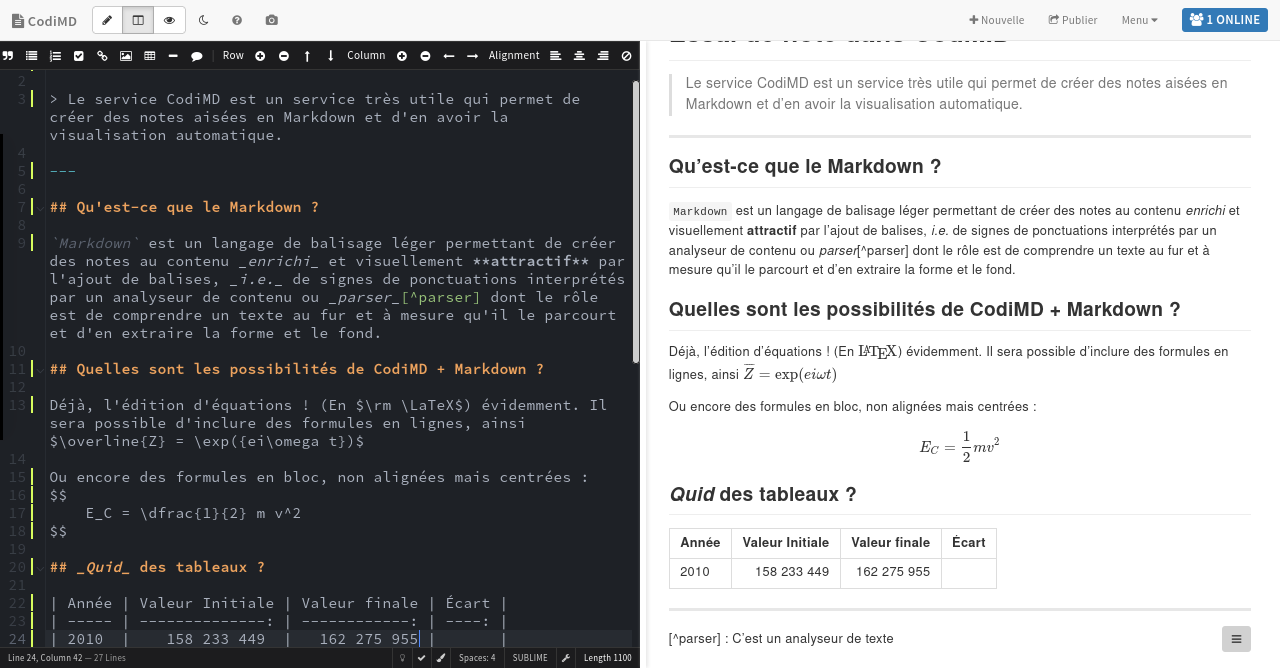
\includegraphics[width=\linewidth]{./Captures/codimd.exemple.png}
	\caption{L'application Codi MD}
\end{figure}

L'exemple montré ci-dessus est typique d'un document \texttt{Markdown} avec de nombreuses options visibles~: les structures hiérarchisées des titres, les emphases fortes et faibles, l'insertion d'éléments mathématiques issus de \LaTeX{} et les premières lignes d'un tableau.

La fenêtre se décompose en deux parties~:
\begin{itemize}
	\item à gauche la partie code, avec, en haut de la demi-fenêtre, quelques icônes permettant de formater ou d'insérer des éléments,
	\item droite, la partie formatée où les modifications se voient.
\end{itemize}

Évidemment, il y a des options de personnalisation dans la barre horizontale grise au dessus des deux demi-fenêtres, permettant d'assombrir, entre autres, la totalité de la fenêtre.